\begin{frame}[c,parent={cmap:software-testing}, hasprev=false, hasnext=false]
\frametitle{Functional testing}
\label{cmap:functional-testing}

\insertcmap{Courses-SoftwareTesting-FunctionalTesting}
\end{frame}



\begin{frame}[parent={cmap:functional-testing}, hasprev=false, hasnext=true]
\frametitle{Functional testing}
\label{concept:functional-testing}

\begin{block:concept}{Functional testing}
Functional testing is a technique in which testing is based solely on the
requirements and specifications.
\end{block:concept}

\begin{block:fact}{Black-box testing}
	\centering
	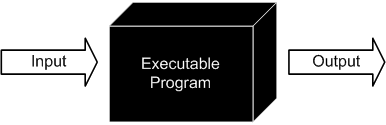
\includegraphics[width=\textwidth]{Functional testing/Black box testing (no requirements)}
\end{block:fact}
\end{frame}


\begin{frame}[hasprev=true, hasnext=true]
\frametitle{Functional testing}
\label{concept:black-box}

\begin{columns}[t]
\column{.6\textwidth}
\begin{block:fact}{Black box}
\begin{itemize}
	\item Functional testing considers the product under test as a box:
	\begin{itemize}
		\item of which are only known its input and outputs;

		\item which may only be visualized from its exterior.
	\end{itemize}

	\item It requires no knowledge of the internal paths, structure, or
	implementation of the software.
\end{itemize}
\end{block:fact}

\column{.4\textwidth}
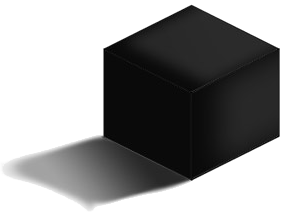
\includegraphics[scale=.3]{Functional testing/Black box}
\end{columns}
\end{frame}



\begin{frame}
\frametitle{Functional testing}
\framesubtitle{Test phases}

\begin{block:fact}{Test phases}
\begin{itemize}
	\item Functional testing can be applied to any test phase.

	\item Functional testing approach remains the same regardless of the size
	and the input/output complexity of the software (unit, module, subsystem)
	under testing.
\end{itemize}
\end{block:fact}


\begin{block:fact}{Test phases}
\begin{itemize}
	\item Actually, software testing of big software pieces forces the tester
	to use functional testing as there are simply too many paths through the
	software to apply other test techniques.
\end{itemize}
\end{block:fact}
\end{frame}


\begin{frame}
\frametitle{Functional testing}
\framesubtitle{Limitations}

\begin{block:fact}{Limitations}
\begin{itemize}
	\item Functional testing depends upon good software requirements
	specification.

	\item Functional testing is not suitable for testing complex processing
	that requires simple input data.
\end{itemize}
\end{block:fact}
\end{frame}



\begin{frame}[hasprev=true, hasnext=false]
\frametitle{Functional testing}

\begin{block:procedure}{Basic steps for functional testing}
\begin{enumerate}
	\item Software requirements are analyzed.
	\begin{itemize}
		\item Valid inputs are chosen based on the software requirements
		to determine that the software processes them correctly.

		\item Invalid inputs must also be chosen to verify that the software
		detects and properly handles them.
	\end{itemize}

	\item Expected outputs for those inputs are determined.

	\item Test cases are constructed with the selected inputs.

	\item The test cases are run.

	\item Actual outputs are compared with the expected outputs, evaluating
	the proper functioning of the software.
\end{enumerate}
\end{block:procedure}
\end{frame}
